\documentclass[8pt]{report}
\usepackage{amsmath, xfrac, enumitem, graphicx, ulem, float, bigints, bm, textcomp}
\usepackage{titlesec, mathtools}
\usepackage[margin=0.7in]{geometry}
\graphicspath{ {images/} }
\linespread{0.8}
\title{\Huge{\textsc{Casting - GATE}}}
\author{\huge{\textbf{Kulasekaran}}}
\begin{document}
\maketitle
\tableofcontents
%-----------------------------------------------------------------------------------------%
\chapter{Metal Casting}
\section{Introduction to Casting}
	\begin{itemize}
		\item Casting - Creating objects by melting metal, pouring it into a cavity that has the shape of that desired object and after solidification of metal, the object is obtained.
		\item Expendable mould - Mould is broken after each object is cast
		\item Permanent mould - Mould is reused for several cast
		\subsection{Advantages}
			\begin{itemize}
				\item Less expensive
				\item Both brittle and ductile objects can be cast
				\item Easier to produce intricate shapes
			\end{itemize}
		\subsection{Disadvantages}
			\begin{itemize}
				\item Dimensional accuracy and Surface finish is very less
				\item Gas defects can form
				\item More labour intensive process
				\item Non-uniform mechanical properties of cast objects due to Non-uniform cooling
			\end{itemize}
	\end{itemize}\hrulefill
%-----------------------------------------------------------------------------------------%
\section{Pattern}
	\begin{itemize}
		\item It is the replica of the desire object with slight modifications like core and allowances. Can be made of Wood, plastic or metal
		\subsection{Shrinkage allowance (+ve)}
			\begin{itemize}
				\item $T_P$ = Pouring Temperature; $T_f$ = Freezing temperature; $T_a$ = Ambient Temperature ($T_P > T_f > T_a$)
				\item \textbf{Liquid Shrinkage} - Metal cools from $T_P$ to $T_f$
				\item \textbf{Solidification Shrinkage} - Cooling during Phase transition at constant temp
				\item \textbf{Solid Shrinkage} - Metal cools from $T_f$ to $T_a$
				\item Liquid and Solidification Shrinkage can be compensated with Riser
				\item Solid shrinkage requires shrinkage allowance
			\end{itemize}\hrulefill
%-----------------------------------------------------------------------------------------%
		\subsection{Draft or Taper allowance (+ve)}
			\begin{itemize}
				\item For easy removal of pattern from sand mould without damaging the mould
				\item x = h$\tan\theta$ (Around 0.5 to 2\textdegree)
			\end{itemize}\hrulefill
%-----------------------------------------------------------------------------------------%
		\subsection{Machining allowance (+ve)}
			\begin{itemize}
				\item Since casting products have poor surface finish, machining is required for cast objects. This reduces the object's dimensions. So, the casting dimension of the object must be more than actual required dimension of the object. 
			\end{itemize}\hrulefill
%-----------------------------------------------------------------------------------------%
		\subsection{Shake or Rapping allowance (-ve)}
			\begin{itemize}
				\item When Pattern is tried to be taken out of the mould, due to shaking, it increases the mould cavity. So, if the cavity dimension was given slightly less compared to the original product dimension, then the shaking itself will bring the cavity to the required dimension
			\end{itemize}\hrulefill
%-----------------------------------------------------------------------------------------%
		\subsection{Distortion or Camber allowance (+ve)}
			\begin{itemize}
				\item V-shape, U-shape and flat object with very less thickness can distort. To avoid distortion, allowance is provided opposite to the direction of distortion
			\end{itemize}\hrulefill
%-----------------------------------------------------------------------------------------%
	\end{itemize}\hrulefill
%-----------------------------------------------------------------------------------------%
\section{Terms}
	\begin{figure}[H]
		\centering
		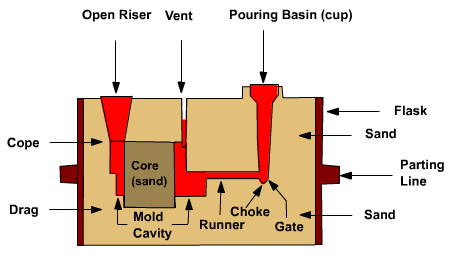
\includegraphics[scale=0.5]{Terms.png}
	\end{figure}
	\subsection{Flask}
		\begin{table}[H]
			\begin{tabular}{cc}
				\parbox{6cm}{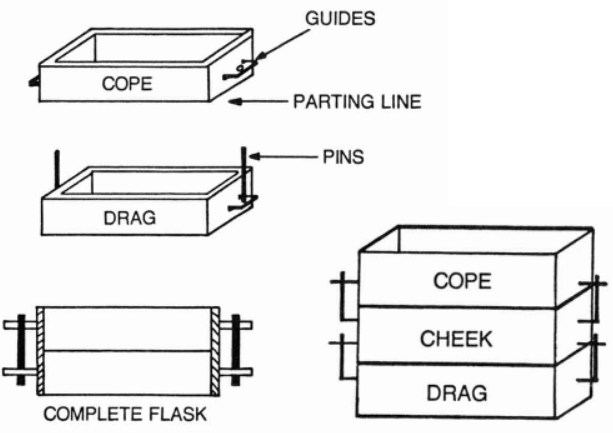
\includegraphics[scale=0.4]{flask.png}} &
				\parbox{15cm}{$\rightarrow$ Holds the sand mould. Flask can be made of Wood or Metal\\\\ $\rightarrow$ \textbf{Cope} - Top part\\\\ $\rightarrow$ \textbf{Drag} - Bottom part\\\\ $\rightarrow$ \textbf{Cheek} - Middle part}
			\end{tabular}
		\end{table}
	\subsection{Core}
		\begin{itemize}
			\item If the desired object has a \textbf{hollow cavity}, then to cast such object, that hollow cavity sized object is placed in the sand mould, so that the molten metal can't fill that space. 
		\end{itemize}
	\subsection{Pouring Basin}
		\begin{itemize}
			\item Funnel shaped cavity at the top of the mould into which the molten metal is poured
		\end{itemize}
	\subsection{Sprue}
		\begin{itemize}
			\item The passage through which the molten metal from the Pouring basin reaches the mould cavity
		\end{itemize}
	\subsection{Choke}
		\begin{itemize}
			\item Regulates flow rate of molten metal and hence prevents defects
			\item Can be created by using core or creating a tapered section in gating system
		\end{itemize}
	\subsection{Runner}
		\begin{itemize}
			\item The passage way in the parting plane. Parting plane is the plane between the top and bottom part of the mould
		\end{itemize}
	\subsection{Difference between Sprue and Runner}
		\begin{itemize}
			\item Sprue is the main and largest channel and is located at a top point.
			\item Runner distributes the molten metal to every gates
		\end{itemize}
	\subsection{Gate}
		\begin{itemize}
			\item Entry point of the mould cavity
		\end{itemize}
	\subsection{Chaplet}
		\begin{itemize}
			\item Used to support core objects and keep them fixed
			\begin{figure}[H]
				\centering
				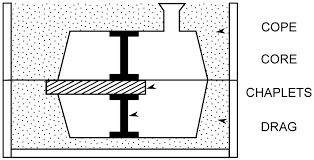
\includegraphics[scale=0.4]{chaplet.png}
			\end{figure}
		\end{itemize}
	\subsection{Chills}
		\begin{itemize}
			\item metalling objects placed inside to increase cooling rate
		\end{itemize}
	\subsection{Riser}
		\begin{itemize}
			\item Acts as a reservoir
			\item When there is reduction in volume of metal in the cavity due to contraction, the molten metal in riser can fill that void. 
		\end{itemize}
	\subsection{Vents}
		\begin{itemize}
			\item Vents are small holes provided for the escape of gases or trapped air pockets and hence preventing gas defects 
		\end{itemize}\hrulefill
%-----------------------------------------------------------------------------------------%
\section{Types of Pattern}
	\subsection{Solid or Single piece pattern}
		\begin{itemize}
			\item Used for simple shapes. 
		\end{itemize}
	\subsection{Split piece pattern}
		\begin{itemize}
			\item Pattern is split into more than one part
		\end{itemize}
	\subsection{Loose piece pattern}
		\begin{itemize}
			\item Used for parts with internal webs, projections, undercuts etc.,
		\end{itemize}
	\subsection{Gated Pattern}
		\begin{itemize}
			\item
		\end{itemize}
	\subsection{Match Plate pattern}
		\begin{itemize}
			\item 
		\end{itemize}
	\subsection{Cope and Drag pattern}
		\begin{itemize}
			\item
		\end{itemize}
	\subsection{Sweep pattern}
		\begin{itemize}
			\item 
		\end{itemize}
	\subsection{Follow board pattern}
		\begin{itemize}
			\item 
		\end{itemize}
	\subsection{Skeleton pattern}
		\begin{itemize}
			\item 
		\end{itemize}\hrulefill
%-----------------------------------------------------------------------------------------%
\section{Properties of Moulding sand}
	\begin{itemize}
		\item
	\end{itemize}\hrulefill
%-----------------------------------------------------------------------------------------%
\section{Core design}
	\begin{itemize}
		\item
	\end{itemize}\hrulefill
%-----------------------------------------------------------------------------------------%
\section{Types of sand}
	\begin{itemize}
		\item
	\end{itemize}\hrulefill
%-----------------------------------------------------------------------------------------%
\section{Additives used in moulding sand}
	\begin{itemize}
		\item
	\end{itemize}\hrulefill
%-----------------------------------------------------------------------------------------%
\section{Types of Moulding methods}
	\begin{itemize}
		\item
	\end{itemize}\hrulefill
%-----------------------------------------------------------------------------------------%
\section{Gating system}
	\begin{itemize}
		\item
	\end{itemize}\hrulefill
%-----------------------------------------------------------------------------------------%
\section{Top Gate}
	\begin{itemize}
		\item
	\end{itemize}\hrulefill
%-----------------------------------------------------------------------------------------%
\section{Bottom Gate}
	\begin{itemize}
		\item
	\end{itemize}\hrulefill
%-----------------------------------------------------------------------------------------%
\section{Parting Line Gate}
	\begin{itemize}
		\item
	\end{itemize}\hrulefill
%-----------------------------------------------------------------------------------------%
\section{Step Gate}
	\begin{itemize}
		\item
	\end{itemize}\hrulefill
%-----------------------------------------------------------------------------------------%
\section{Solidification Time}
	\begin{itemize}
		\item
	\end{itemize}\hrulefill
%-----------------------------------------------------------------------------------------%
\section{Types of Solidification}
	\begin{itemize}
		\item
	\end{itemize}\hrulefill
%-----------------------------------------------------------------------------------------%
\section{Purpose of Riser}
	\begin{itemize}
		\item
	\end{itemize}\hrulefill
%-----------------------------------------------------------------------------------------%
\section{Classification of Casting Techniques}
	\begin{itemize}
		\item
	\end{itemize}\hrulefill
%-----------------------------------------------------------------------------------------%
\section{Permanent moulds}
	\begin{itemize}
		\item
	\end{itemize}\hrulefill
%-----------------------------------------------------------------------------------------%
\section{Casting Defects}
	\begin{itemize}
		\item
	\end{itemize}\hrulefill
%-----------------------------------------------------------------------------------------%
\section{Cupola}
	\begin{itemize}
		\item
	\end{itemize}\hrulefill
%-----------------------------------------------------------------------------------------%
\section{Non-Destructive Testing}
	\begin{itemize}
		\item
	\end{itemize}\hrulefill
%-----------------------------------------------------------------------------------------%
\section{Visual Inspection}
	\begin{itemize}
		\item
	\end{itemize}\hrulefill
%-----------------------------------------------------------------------------------------%
\section{Hammer Test}
	\begin{itemize}
		\item
	\end{itemize}\hrulefill
%-----------------------------------------------------------------------------------------%
\section{Radiography}
	\begin{itemize}
		\item
	\end{itemize}\hrulefill
%-----------------------------------------------------------------------------------------%
\section{Liquid Penetrant test}
	\begin{itemize}
		\item
	\end{itemize}\hrulefill
%-----------------------------------------------------------------------------------------%
\section{Ultrasonic Inspection}
	\begin{itemize}
		\item
	\end{itemize}\hrulefill
%-----------------------------------------------------------------------------------------%
\end{document}
%-----------------------------------------------------------------------------------------%
%-----------------------------------------------------------------------------------------%
%-----------------------------------------------------------------------------------------%
